\documentclass[a4paper,listof=totoc,toc=sectionentrywithdots,abstract=false]{scrartcl}
\usepackage[affil-it]{authblk}

\usepackage{graphicx}
\usepackage[ngerman,english]{babel}
\usepackage{textcmds}
\usepackage{float}
\usepackage{csquotes}
\usepackage{tabularx}
\usepackage{pifont}% http://ctan.org/pkg/pifont

\newcommand{\cmark}{\ding{51}}%
\newcommand{\xmark}{\ding{55}}%

\usepackage[
backend=biber,
%style=chicago-authordate,
%citestyle=chicago-authordate,
%style=numeric,
%citestyle=numeric,
%style=authoryear,
%citestyle=authoryear,
style=alphabetic,
citestyle=alphabetic,
maxnames=1,
maxalphanames=1,
]{biblatex}

\renewcommand*{\labelalphaothers}{}

\DefineBibliographyStrings{english}{%
	andothers = {\em et\addabbrvspace al\adddot}
}

\addbibresource{biblatex.bib} %Imports bibliography file
\usepackage[colorlinks=false,hidelinks]{hyperref}

%\titlefoot{\centering\includegraphics[width=6cm]{images/title}}
\title{Interpolation - Heat island effect on the example of Berlin}
\subtitle{FOSSGIS Seminar 2020}
\date{\today}
\author{Anja Doppelmayr \& Malte Heinzelmann}
\affil{Ruprecht-Karls-Universit\"at Heidelberg}
\graphicspath{images/}

\begin{document}

\maketitle

%{\centering\includegraphics[width=6cm]{images/title}}

\begin{abstract}
	\setlength{\parindent}{0pt}
	% !TeX root = ../document.tex

\noindent\textbf{Abstract.} The "Intra-Urban Heat Island Effect" describes the phenomenon that certain urban areas experience higher heat accumulation - und thus temperatures - over the course of a day than other areas, such as natural landscapes or open water due to the absorption and re-emittance of infrastructure such as buildings, roads and artificial or sealed surfaces.

Increased heat islands within the city have a negative effect, not only on ecosystems, but on people’s health and well-being especially for the vulnerable populations e.g. infants and elderly people. Hence, the heat islands effect should be considered during city planning activities.

The goal for this project is to analyze temperature data in Berlin to identify possible locations of heat islands and their development during a day. Raw data was obtained from the citizen science project openSenseMap\footnote{\url{https://opensensemap.org/}}, aggregated into ten-minute average measurements and used to interpolate a series of stations within the boundaries of Berlin. The final product - an animation of the temperature over the course of a day - will be beneficial for planning authorities and in developing measures to counteract urban heat islands.

\end{abstract}

%\pagebreak
%\tableofcontents
\pagebreak
% !TeX root = ../document.tex

\section{Introduction}

The basic definition of an urban heat island (UHI) effect is \ldq{}[...] that an urban area or metropolitan area is significantly warmer than its surrounding rural areas due to human activities\rdq{} \cite{takebayashi_chapter_2020}. Higher temperatures than those in the surrounding areas can indicate heat islands. As known, infrastructure such as buildings, roads, etc. absorb and re-emit the sun’s radiation in the form of heat, whereas natural landscapes such as forests and water bodies have a cooling effect. \cite{us_epa_learn_2014}

Thus, replacing natural areas with dense concentrations of buildings, infrastructure, pavements and other sealed surfaces that absorb and retain heat, leads to an increase in air temperature in urban areas relative to their rural counterparts. This effect, however, is not only comprehensible when comparing a metropolitan area to its surrounding, more natural realm, but also within a city itself. 

Temperature differences within urban areas are so-called \ldq{}Intra-Urban Heat Islands (IUHI)\rdq{}. \cite{bruns_stable_2017}
These heat islands within the city have a negative effect, not only for people’s health, well-being and comfort - especially in regard to the vulnerable population – but also for infrastructure, urban ecosystems and the living environment. Moreover, increased heat stress has been found to be the source for higher energy demands (for cooling) and the degradation of air quality in urban areas. \cite{mohajerani_urban_2017}

\subsection{Project Goals}

The fundamental aim of our study is to analyze temperature data in order to be able to create a visual product of the intra-urban heat islands effect, by making this effect and it's development throughout the day visible. Subsequently, the final animation can be used to support planning authorities. Current developments in regard to climate change urge the implementation of countermeasure as well as mitigation strategies in urban areas, where more greening is obviously needed. \cite{ketterer_comparison_2015}

Fostering measures such as cool and reflective pavements, green spaces and air circulation systems \cite{mohajerani_urban_2017} can be supported by preparing material, which helps to identify areas of increased heat stress and evaluated where countermeasures need to be implemented.

Our approach, therefore, includes the comparison of changes in air temperature over the course of the warmest day in 2019 (25.7.) and 2020 (9.8.) in Berlin. The study area is defined by Germany’s capital city Berlin. This site was chosen due to the availability of various data points and measurements in regard to our main source of data: openSenseMap (see section \ref{sec:data}). Furthermore, we hope to find a more significant intra-urban heat islands effect, as compared to other areas in Germany, merely because of the size and a relatively high degree of sealed surfaces. \cite{gdv_munchen_2018} Although the effect should be identifiable in similar urban areas, the comparison of different interpolation methods stands in the focus of this project, which is why we decided to use a more self-evident study site. Thus, the result of the comparison of the different methods below should point towards one overall method, which is best-suitable for answering questions in relation to the IUHI effect. 

\subsection{Data: Selection and preparation (workflow)}
\label{sec:data}

Typically, the UHI effect is measured by the temperature difference between a city and its surrounding area.\cite{us_epa_learn_2014} In a study from 2012, the authors used land use/land cover, soil texture, and a digital elevation model as independent variables for interpolating and predicting temperature data in an area with a limited number of stations.\cite{samanta_interpolation_2012} As our study site did show various stations where temperature was measured on a regular basis, we were able to use this data directly and were hence not dependent on predicting point data based on independent variables. While our data did not demand for a series of different factors, but accurate and \ldq{}clean\rdq{} temperature data, the main preparation work was dedicated to extracting useful data, averaging the temperatures and selecting relevant sensor types (discussed below). Consequently, our temperature data is limited by the ultimate measurements of the different stations, their reliability and accuracy, which can be influenced by immediate surroundings or technical failure (also discussed in section \ref{sec:discussion}). Thus, if we would bring different variables, like elevation, solar radiation, wind speed and direction, distance to natural (vegetated and water) and artificial surfaces etc. into play, then the results and statements could be more accurate. With respect to time and thematic priority, this would, however, be outside the scope of this project.

Due to the fact, that openSenseMap is a citizen science project, not all stations will provide data of equal quality. The question, if temperature data derived from openSenseMap alone is representative for visualizing IUHI, is also a question of selecting a specific time-frame. Our central goal is to use the methods of interpolation to show local temperature variations and - after further analysis - be able to identify areas with higher concentrations of heat stress. The end product is aimed at generating an animation of these results. Based on these objectives and the fact that an analysis of temperature variability over a longer period of time would require large amounts of data, we decided to focus on the daily variation of the IUHI for the two selected days within the last two years, as mentioned before.

For the preparation of the data sets we had to take a few preliminary steps and explore the data at hand. For this purpose, we downloaded raw data from \url{https://opensensemap.org/} and aggregated the temperature data for the hottest day of the year 2019 and 2020, the 25.07 and 09.08 respectively. The initial number of stations downloaded from opensensemap.org resulted in 86 for 2019 and 121 for 2020 respectively. However, as some stations lacked data values for the necessary (10-minute-average) time intervals of the selected days, these had to be filtered. In a next step, a selection was made based on the double standard deviation – outliers were removed and the final data set consisted of 73 and 88 stations.

Furthermore, the sensor descriptions posed a problem as the type of measurement is a free-text field, thus allowing contributors to specify the type freely. The API endpoint (\url{/boxes/data}) requires the user to specify a phenomenon name within the request. Therefore, only the most common name \ldq{}Temperatur\rdq{} was used.

The final product used for further analysis consisted of a collection of stations and their aggregated measurements for each day.


\begin{figure}[b!]
	\centering
	\scalebox{0.85}{
		\begin{tikzpicture}[node distance = 2cm, auto, every node/.style={color=text, fill=background, font=\sffamily}, align=center]
			% Place nodes
			\node [block] (in) {openSenseMap};
			\node [cloud, right=1.6cm of in, text width=7em] (avg) {Average\\into 10 minute intervals};
			\node [cloud, right=1.6cm of avg, text width=8em] (filter) {Filter\\by std deviation};
			\node [decision, below=1.6cm of filter] (interpolate) {Interpolate};
			\node [cloud, left=1.6cm of interpolate, text width=8em] (colorize) {Colorize\\1-band Tiff $\Rightarrow$ 4-band RGBA Tiff};
			\node [block, below=2.3cm of in] (out) {Generate frame};
			% Draw edges
			\draw [->] (in) -- (avg);
			\draw [->] (avg) -- (filter);
			\draw [->] (filter) -- (interpolate);
			\draw [->] (interpolate) -- (colorize);
			\draw [->] (colorize) -- (out);
		\end{tikzpicture}
	}
	\caption{Project workflow overview}
	\label{fig:workflow}
\end{figure}



% !TeX root = ../document.tex

\section{Interpolation methods}

The following chapter describes interpolation in general with regard to the most frequently used methods. We will give an introduction to the background of each method, their suitability/advantages and disadvantages as well as examples of application in other studies. Furthermore, we present possibilities of carrying out interpolation analysis and an overview of which methods are supported by a variety of FOSSGIS tools.


\subsection{Statistical and Deterministic methods?}

A deterministic method always generates the exact same output for a given input. Thus, leading to reproducible results, whereas a statistical method might not generate the same results.
% TODO: Should we keep this?

\subsection{What is spatial interpolation?}

Spatial interpolation is the calculation of nearby and unknown values on the basis of neighboring known values \cite{gitta_raumliche_2016}. Interpolation methods are often used for analyzing spatial and spatio-temporal distributions of physical but also socioeconomic phenomena. These phenomena can be approximated by certain functions, which are location dependent within space \cite{mitas_spatial_1999}. Interpolation is thus very useful for estimating or predicting missing geographic point data, such as elevation, rainfall, chemical concentrations, noise levels etc. \cite{samanta_interpolation_2012}. Calculating these unknown values is done via a series of different methods, where the methods themselves again depend on the research question and the data present. In this study we will be focusing on temperature data only and give a short overview of similar studies and their choice of method.

\subsection{The diversity of methods}

In this chapter, we will give a short introduction to the various methods, starting off with a general possibility of classification – a schematic overview. According to \citeauthor{hofstra_comparison_2008} the choice of method, when interpolating climate-related data, depends primarily on the different variables, station densities and climate regimes. It is rather difficult to find a single method which fulfills all requirements. Thus, the goal is to give an overview of different (and widely used) interpolation methods (mostly in the context of climate-related research) and present some advantages and disadvantages of each method as well as give some examples of their application.

\subsection{Schematic overview}

Generally, there is a difference between global and local interpolation, whereas global interpolation is not suitable for determining values that are as exact as possible, but for assessing rough global spatial structures. \cite{gitta_raumliche_2016}
Interpolation methods are also distinguishable in exact and non-exact or gradual and abrupt interpolation (see figure \ref{fig:exact_non_exact_interploation}). In Figure 1 below (left), the generated surface, which stands for the resulting interpolation, fits exactly to the data points, although the surface has abrupt  \ldq{}steps\rdq{} (the used method here is Natural Neighbor interpolation). Adjusting the interpolation surface results in a smoother surface, as seen in figure \ref{fig:exact_non_exact_interploation} on the right.
The inverse distance weighting (IDW) method depicted here, does not follow the high and low data points exactly, which is why a \ldq{}moving average\rdq{} or \ldq{}smoothing\rdq{} of the data occurs. In the end, the choice depends on whether  \ldq{}[...] we need the interpolated surface to exactly pass through the data points or we require a surface which simply represents the general trend\rdq{}. \cite{wyatt_interpolation_nodate}



\begin{figure}
	\begin{minipage}[b]{.48\linewidth}
		\includegraphics[width=\linewidth]{images/exakte_interpolation.jpg}
	\end{minipage}
	\hfill
	\begin{minipage}[b]{.48\linewidth}
		\includegraphics[width=\linewidth]{images/nicht_exakte_interpolation.jpg}
	\end{minipage}
	\caption{Different interpolation surfaces due to exact (left) and non-exact (right) interpolation\cite{gitta_raumliche_2016}}
	\label{fig:exact_non_exact_interploation}
\end{figure}

And finally, we can differentiate between deterministic and stochastic methods.\cite{gitta_raumliche_2016}
Deterministic methods encompass for example \ldq{}TIN\rdq{}, \ldq{}IDW\rdq{} or \ldq{}Spline\rdq{}. \cite{wasser_going_2020} Deterministic interpolation techniques are generally based on precisely predictable (= deterministic) spatial relationships, whereas stochastic (also called probabilistic or geostatistical) methods, make use of underlying statistical properties of the point data. Latter requires advanced knowledge, which is why will focus primarily on deterministic methods. One of the most prominent and important stochastic methods is Kriging.

In regard to suitability, we refer to figure \ref{fig:interpolation_methods_strengths}, which gives a good overview for several of the methods and their advantages and disadvantages. As the choice of method is, as already stated, dependent on the question one poses and the data available, no general statement can be given.


\begin{figure}[b!]
	\includegraphics[width=\linewidth]{images/interpolation_methods_strengths.png}
	\caption{Strengths of interpolation methods \cite{wasser_going_2020}}
	\label{fig:interpolation_methods_strengths}
\end{figure}

\subsection{Common methods}

In a study by \citeauthor{wenjing_cao_study_2009}, the authors compared different interpolation methods for temperature values in China. Their results show that Kriging-exponential and Kriging-spherical methods are the best, or most accurate, interpolations methods, the interpolation precision of IDW is second, but, overall, Kriging-Gaussian and Spline interpolation methods have the lowest accuracy. \cite{wenjing_cao_study_2009} Other studies also show a similar application and result of comparing these methods: 
\citeauthor{hofstra_comparison_2008} compares the methods Natural Neighbour, Kriging and (thin plate) Splines. They conclude that global Kriging is best suitable for a daily climate data set. Also \citeauthor{samanta_interpolation_2012} use the three common methods IDW, Kriging and Spline to estimate climate variables and temperature.
We have, therefore, decided to focus on the four methods: TIN, IDW, Kriging and Spline. We will present these methods shortly, give some examples of usage and their pros and cons.

\subsubsection{TIN}

TIN stands for \ldq{}Triangulated Irregular Network\rdq{}. Hereby, scattered points are linked into a set of triangles, based on so-called Voronoi diagrams (which are the basis for nearest neighbor interpolation). Voronoi diagrams split up a plane into smaller regions, called cells, based on a set of known points (see figure \ref{fig:voronoi_delauny}(a)). In order to derive the geometric construction for TIN, which is called “delaunay triangulation” \cite{sambridge_geophysical_1995}, neighbors within cells that share a common boundary are connected. This is done through the creation of circumcircles of always three known points, which then form a valid triangle. The three nodes, or nearest neighbours, are then taken for the interpolation of each value within an identified triangle, based on their linear relationship \cite{lam_spatial_2009}. Thus, delauny triangulations, which are supported by the linear interpolation algorithm of the GDAL tool, form a surface of non-overlapping triangles \ref{fig:voronoi_delauny}(b)). 


\begin{figure}
	\includegraphics[width=\linewidth]{images/voronoi_delauny.png}
	\caption{(a) Voronoi diagram and corresponding (b) Delaunay triangulation\cite{sambridge_geophysical_1995}}
	\label{fig:voronoi_delauny}
\end{figure}

TIN is commonly used to produce contour maps and also shaded relief maps. \cite{lam_spatial_2009}
It should be noted that there are several ways of constructing the triangulation with the same set of points – thus, comparability is restricted. This method also results in sharp edges, and it is not recommended for analysis of the areas outside the selected data points. \cite{qgis_11_2021} Certainly, TIN is a popular method, which is available with most FOSSGIS tools. 

\subsubsection{Inverse Distance Weighting (IDW)}
IDW is a method whereby the distance between a predicted point and sample point is weighted. More precisely, \ldq{}[t]he sample points are weighted by the inverse of their distance to the predicted point\rdq{} \cite[p.2]{wenjing_cao_study_2009}, which simply means that more weight is given to nearby points than to points in the distance. \cite{lam_spatial_2009} This encompasses Tobler’s well-known assumption that \ldq{}[...] things that are close to one another are more alike than those that are farther apart\rdq{}. \cite{samanta_interpolation_2012}

The IDW method is not only very common, but easily implemented and rather flexible. It is also available for almost any FOSSGIS, but has some shortcomings. A disadvantage of the method is that it does not reproduce the local shape implied by data, but local extrema at the data points (see figure \ref{fig:dem_mitas}). \cite{mitas_spatial_1999} \citeauthor{lam_spatial_2009} points out that the method is, unfortunately quite easily affected by a possible uneven distribution of data points. Even if points are clustered, they will be assigned an equal weight (ibid.). Thus, if data points are following a certain trend, IDW will average it out. 
Overall, the IDW method allows for fast calculations, while different distances are integrated in the calculation and estimation of the missing values. \cite{gitta_raumliche_2016} The method is suitable for dense and equally distributed data points. \cite{wasser_going_2020} IDW is for example beneficial for phenomena such as noise, where the data distribution is correlated with distance. \cite{gis_resources_choosing_2013}

\begin{figure}
	\includegraphics[width=\linewidth]{images/dem.png}
	\caption{Interpolation of a DEM and the result using (a) Voronoi polygons (b) TIN linear interpolation (c) IDW (d) Kriging and (e \& f) Spline (f includes smoothing) \cite{mitas_spatial_1999}}
	\label{fig:dem_mitas}
\end{figure}


\subsubsection{Kriging}

Kriging is a geostatistical approach with many variations. It is a complex interpolation, where it is assumed that \ldq{}[...] the distance or direction between sample points reflects a spatial correlation that can be used to explain variation in the surface\rdq{}. \cite[p.11605]{elumalai_spatial_2017} The method depends on weighting the measured points, the spatial relationships among the measured points around the predicted location, and the distance to the predicted location. \cite{wenjing_cao_study_2009}

Kriging, and other geostatistical approaches, have the capability of producing a prediction surface, and they can also provide some measure of certainty or accuracy of the predicted values. \cite{samanta_interpolation_2012} As (global) Kriging can exceed the known value range (not bound by minima and maxima), but does not pass through any of the sample points, the method is one of the best for all climate variables except maximum temperature. \cite{gis_resources_choosing_2013}

Even with a small number of sample points, Kriging will result in more accurate estimates than IDW. \cite{lam_spatial_2009} The advantage of this particular method is, as already mentioned, that it “[...] delivers a measure of confidence of how likely that prediction will be true” with an error estimation and a confidence interval for every unknown point. \cite{lam_spatial_2009} According to studies evaluated by \citeauthor{hofstra_comparison_2008}, (universal) Kriging is best suitable for interpolating mean precipitation and temperature, as well as daily climate variables. 

\subsubsection{Spline}

Spline is, like IDW, a deterministic method, which estimates missing values based on a mathematical function. The method minimizes overall \ldq{}surface curvature\rdq{} and results in a relatively smooth surface (compare with figure \ref{fig:dem_mitas}), passing exactly through the known data points. \cite{samanta_interpolation_2012} That means, a curved surface is adjusted to the sample points of the dataset. \ldq{}Imagine stretching a rubber sheet across your points and gluing it to each sample point along the way -- what you get is a smooth stretched sheet with bumps and valleys\rdq{} (as shown in figure \ref{fig:spline}). \cite{wasser_going_2020}

In comparison to TIN \& IDW, spline can also estimate data values outside the range of the given data points. Just like TIN, its surface will fit through the data points, unlike IDW or kriging methods (compare with figure \ref{fig:interpolation_methods_strengths}). In a dataset, where points are close together and have large value differences, spline is a disadvantage, especially for slope calculations as it can result in over- and underestimations. \cite{wasser_going_2020} Because spline interpolation smooths out abrupt or \ldq{}edgy\rdq{} changes in values, the method is not suitable, if these characteristics should remain preserved.

\begin{figure}
	\centering
	\includegraphics[width=.5\linewidth]{images/spline.png}
	\caption{Spline \ldq{}rubber sheet\rdq{} fit to known data points \cite{albrecht_spline_2005}}
	\label{fig:spline}
\end{figure}


\subsection{FOSSGIS Implementations}

Table \ref{tab:fossgis_support} gives an overview over the (native) support for the mentioned interpolation methods in different FOSSGIS Tools.

\begin{table}[H!]
	\centering
	\begin{tabular}{c|c|c|c|c}
		Interpolation method & QGIS & GRASS GIS & SAGA & GDAL\\
		\hline
		Nearest neighbor & \xmark &\cmark &\cmark & \cmark \\
		\hline
		TIN & \cmark &\cmark &\cmark & \cmark \\
		\hline
		IDW & \cmark &\cmark &\cmark & \cmark \\
		\hline
		Spline & \xmark &\cmark &\cmark & \xmark \\
		\hline
		Kriging & \xmark &\cmark &\cmark & \xmark \\
	\end{tabular}
	\caption{\label{tab:fossgis_support}FOSSGIS interpolation support}
\end{table}








% !TeX root = ../document.tex

\section{Results}

Within this section we will present the differences in the results of the aforementioned interpolation methods and different implementations. For reference figure \ref{fig:result_berlin} shows all stations used in the following images, their respective temperature on the 9th August 2020at 12:00 and the surface class according to OpenStreetMap data.

The results will be analyzed by visual differences and overall level of accuracy towards the research question. First, we are going to take a look at the visual differences and compare the resulting images of the different interpolation methods, as well as the results of the same methods calculated with the help of different FOSSGIS implementations.

\begin{figure}[H]
	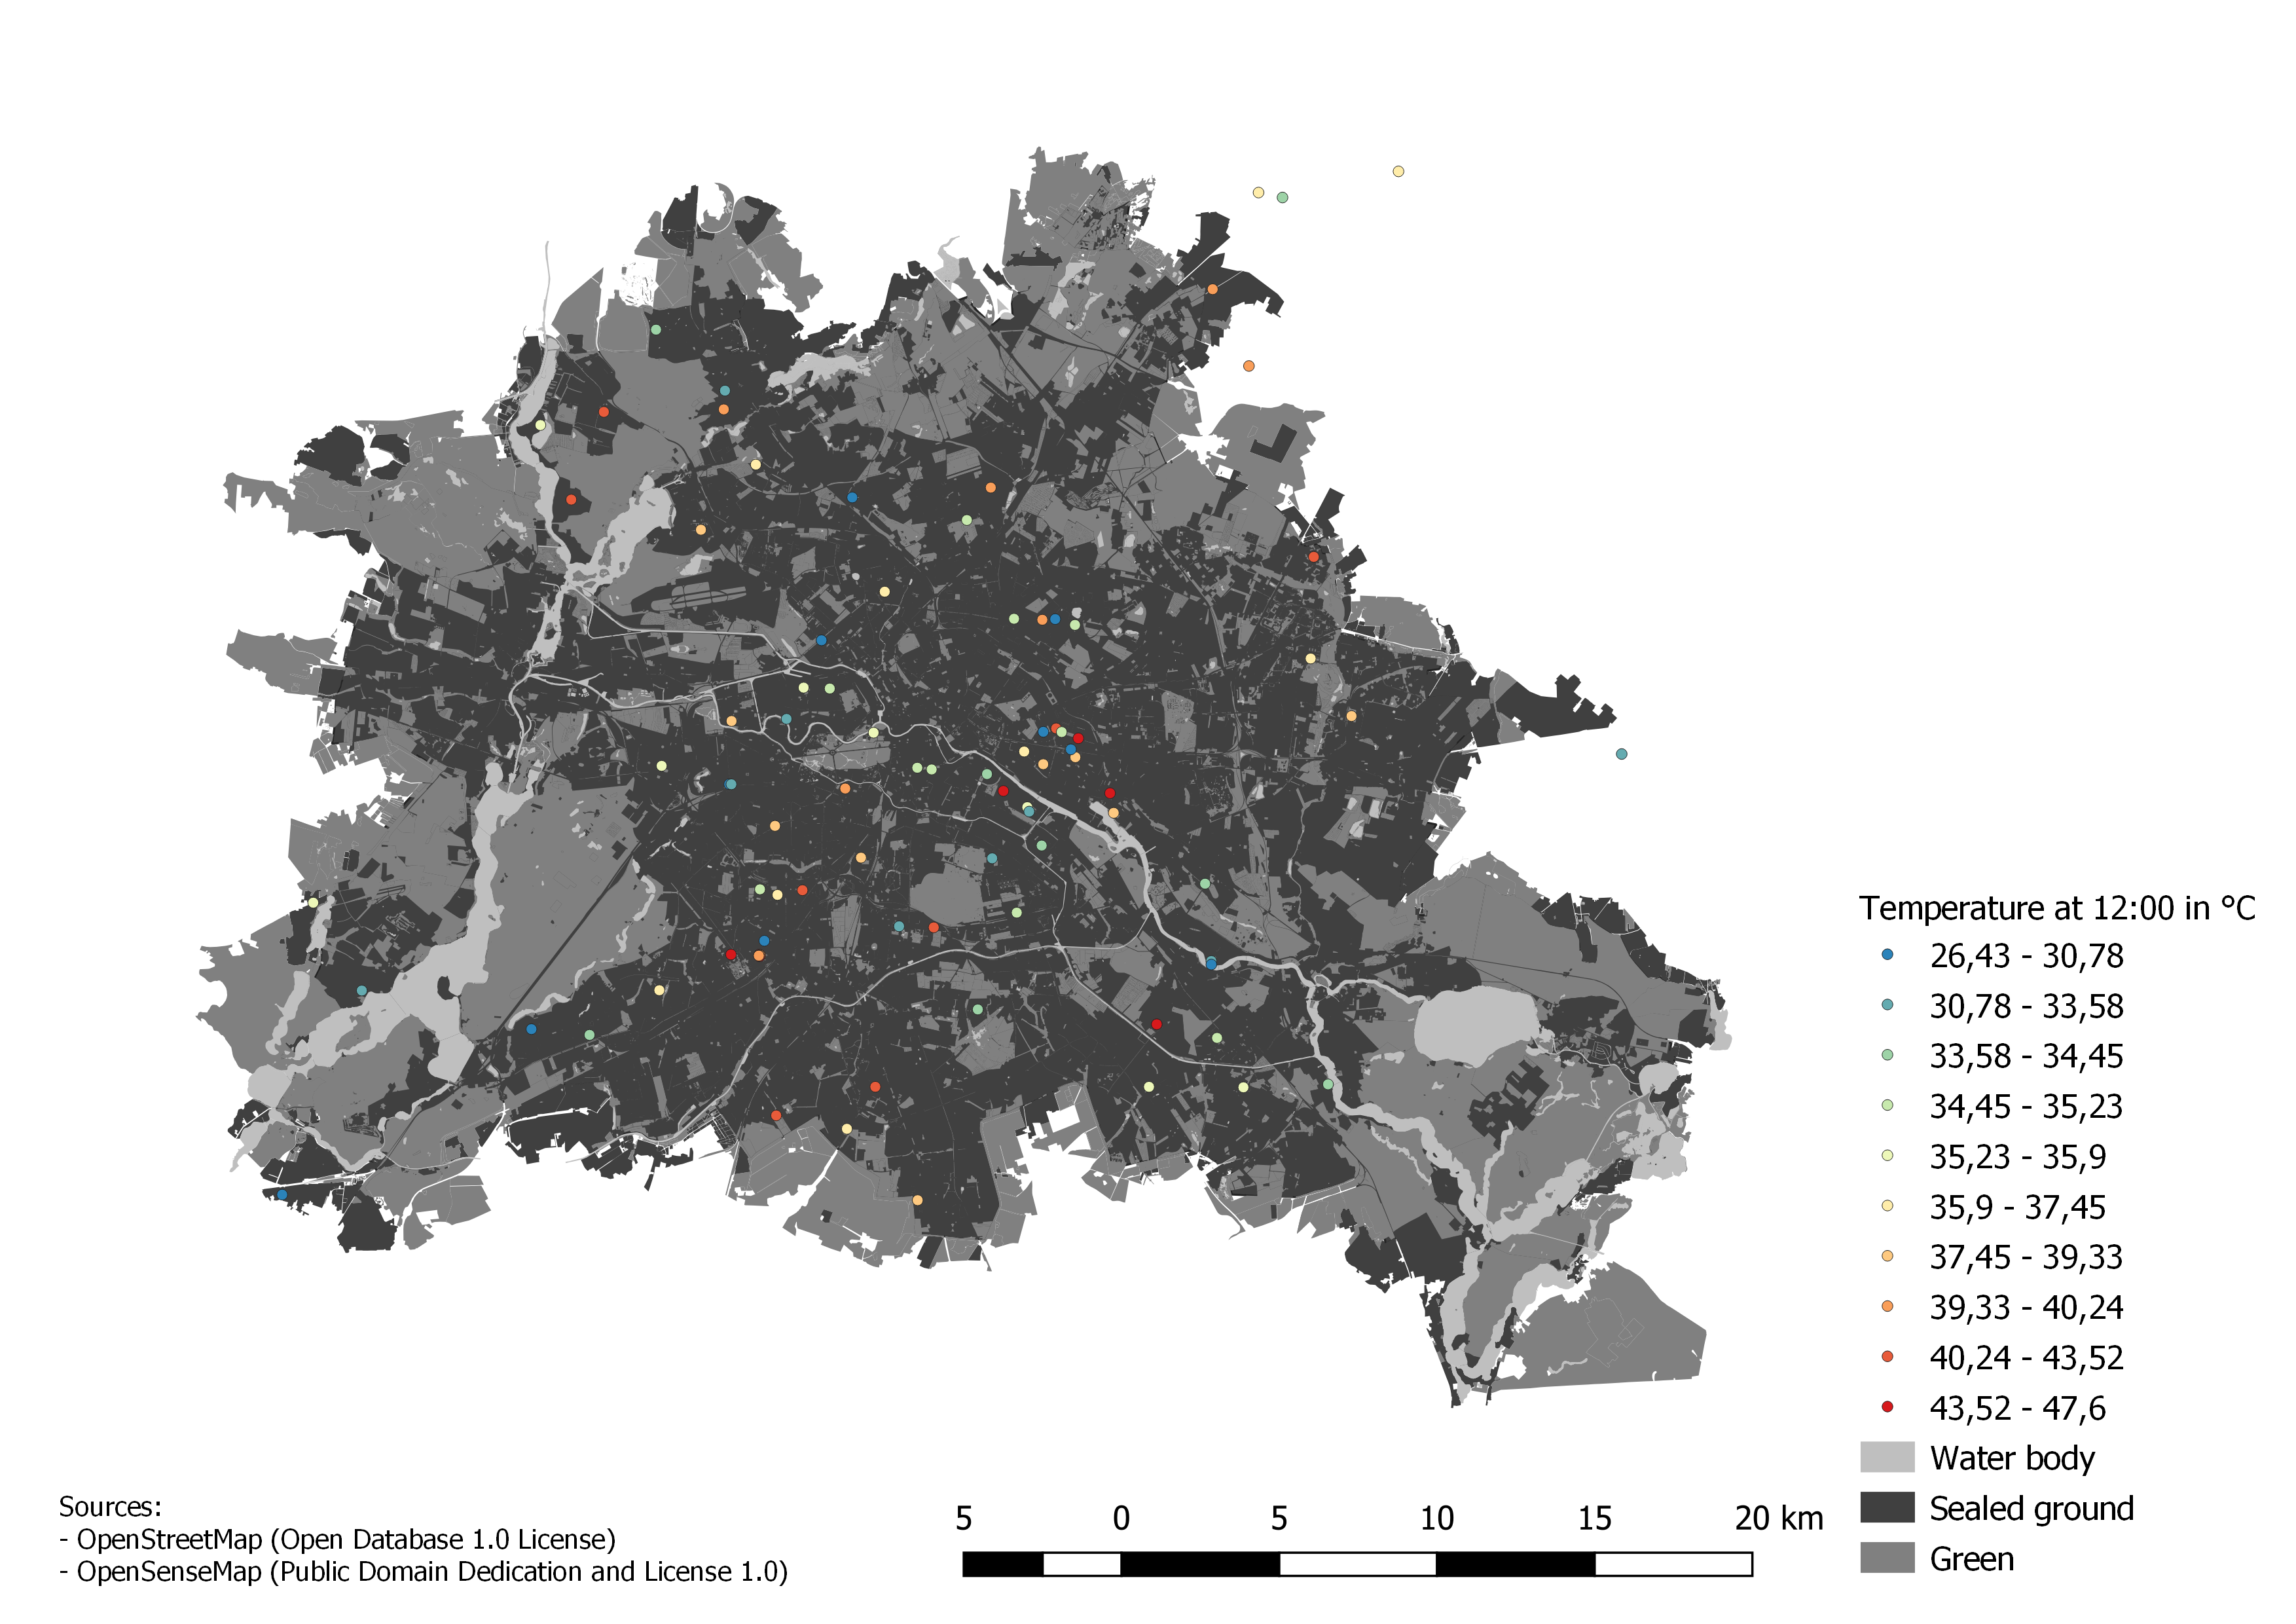
\includegraphics[width=\linewidth]{comparison/berlin.png}
	\caption{Surface types and sensor locations in research area}
	\label{fig:result_berlin}
\end{figure}

\subsection{Nearest neighbor}

The method \ldq{}nearest neighbor\rdq{} is displayed by smaller regions (cells) with sharp edges  (see figure \ref{fig:result_nearest}). Its distinctive visual characteristics do no give sophisticated information about the temperature distribution within the city of Berlin. The geometric shapes of the regions only give a general idea of where the heat islands are, but it does not allow a detailed analysis of the effect nor give a precise location/center of the heat.

\begin{figure}
	\centering
	\subfloat[\centering Nearest neighbor interpolation using GDAL\label{fig:result_nearest}]{{\includegraphics[width=.48\linewidth]{images/interpolation_nearest.png} }}
	\hfill
	\subfloat[\centering TIN interpolation using GDAL\label{fig:result_linear}]{{\includegraphics[width=.48\linewidth]{images/interpolation_tin.png} }}
	\caption{Nearest neighbor and TIN interpolation using GDAL in comparison}
	\label{fig:result_nearest_linear}
\end{figure}


\subsection{TIN interpolation}

Figure \ref{fig:result_linear} shows the TIN interpolation. Hereby visible is the characteristic surface made of triangles and the sharp edges. Due to visual examination the underlying calculation based on the relationship with the nodes of the triangles are apparent. The IUHI is not sufficiently depicted and is not very detailed and therefore does not provide enough information. The fact that TIN interpolation was used to create the image can easily be seen due to the visible convex hull.


\subsection{IDW interpolation}

For the IDW interpolation, GDAL and GRASS GIS were used in order to be able to compare the results. Visually, IDW is recognizable by the \ldq{}Bull Eyes\rdq{}-effect. These are concentric areas of equal values, which ​can be seen around the known points or stations. Compared to th nearest neighbor and TIN interpolation methods, IDW gives a much more detailed output and allows for distinctive analysis of the temperature distribution. Both results calculated with GDAL and GRASS give similar results as shown in figure \ref{fig:result_idw_gdal_grass}. Although the prominent points are fairly similar, differences can be seen in more sparsely covered areas.

\begin{figure}
	\centering
	\subfloat[\centering IDW interpolation using GDAL\label{fig:result_idw_gdal}]{{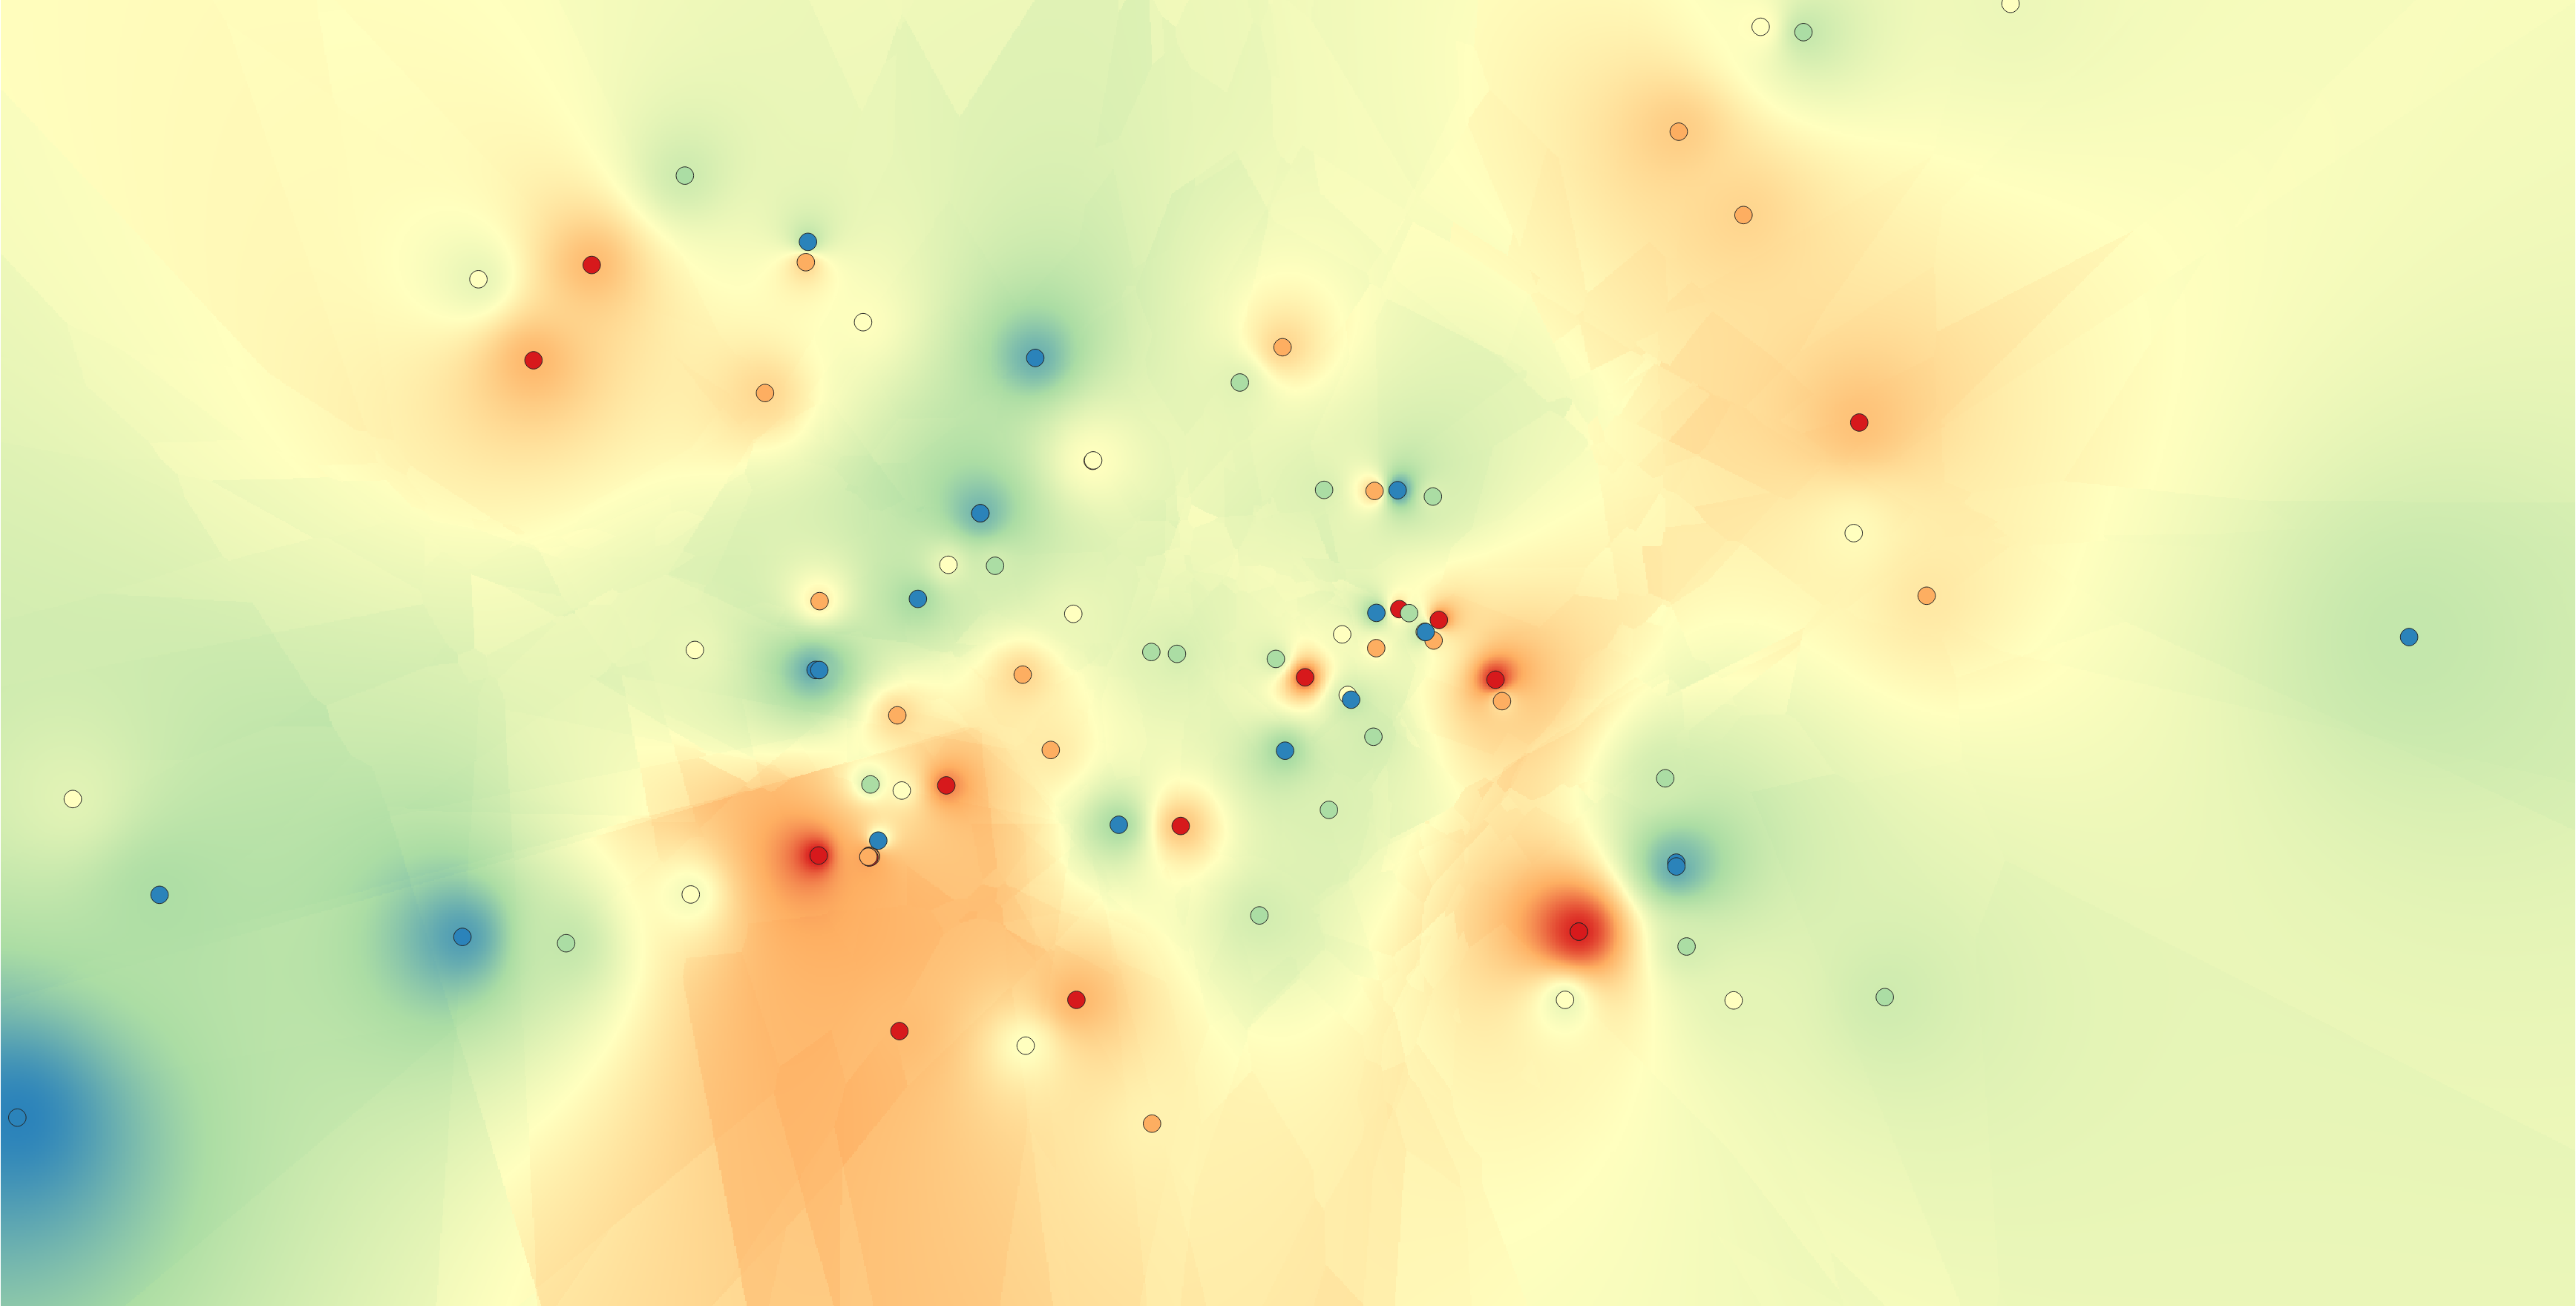
\includegraphics[width=.48\linewidth]{comparison/compare_idw_gdal.png} }}
	\hfill
	\subfloat[\centering IDW interpolation using GRASS GIS\label{fig:result_idw_grass}]{{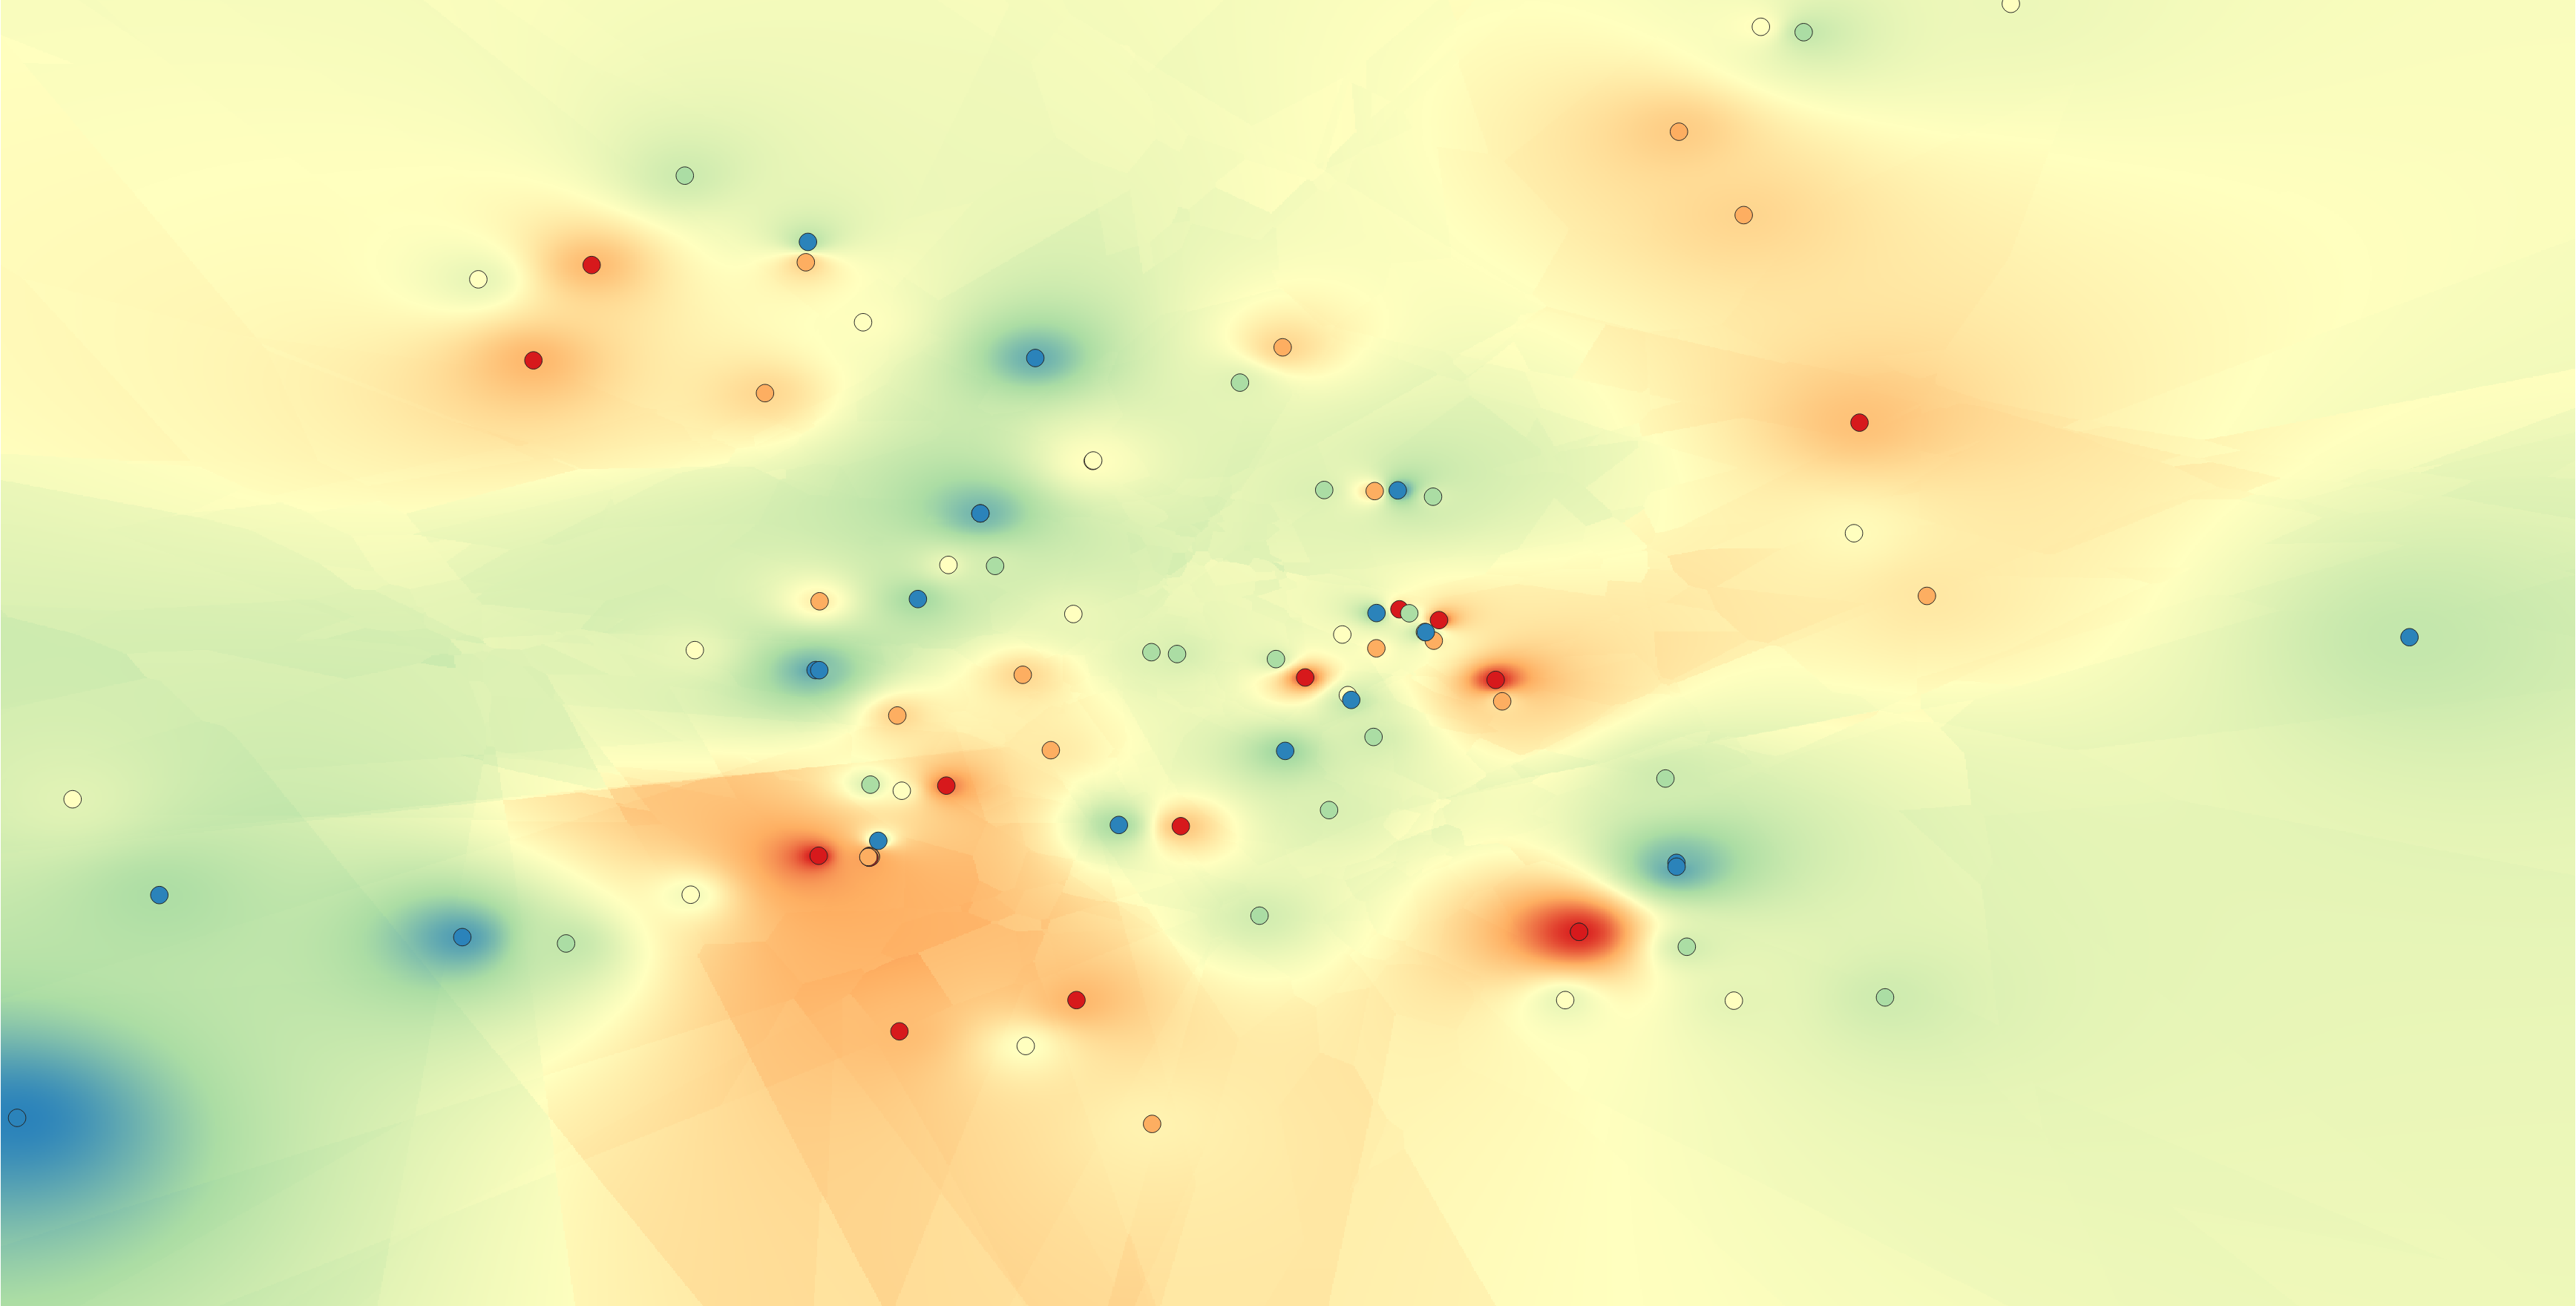
\includegraphics[width=.48\linewidth]{comparison/compare_idw_grass.png} }}
	\caption[Comparison of IDW interpolation between GDAL and GRASS GIS]{Comparison of IDW interpolation between GDAL and GRASS GIS, both using 12 max neighbors and a power factor of 2}
	\label{fig:result_idw_gdal_grass}
\end{figure}

\subsection{B-Spline interpolation}

As SAGA GIS also offers the possibility to interpolate point data, we conducted a B-Spline approximation. SAGA was identified as being one of the least accurate methods as illustrated by \citeauthor{wenjing_cao_study_2009}. As argued before, data points, which are not evenly distributed and have large value differences could pose a problem for spline interpolation. The result seems to have been \ldq{}smoothed\rdq{} out heavily and thus display a very homogeneous data surface. Figure \ref{fig:result_bspline} show that temperature distributions have farther reaching impact (compare lower left corner as well as the rightmost station with IDW). The smoothness can be seen on multiple clusters where the IDW interpolation creates islands that aren't interconnected and have more fringed edges.

\begin{figure}[H]
	\centering
	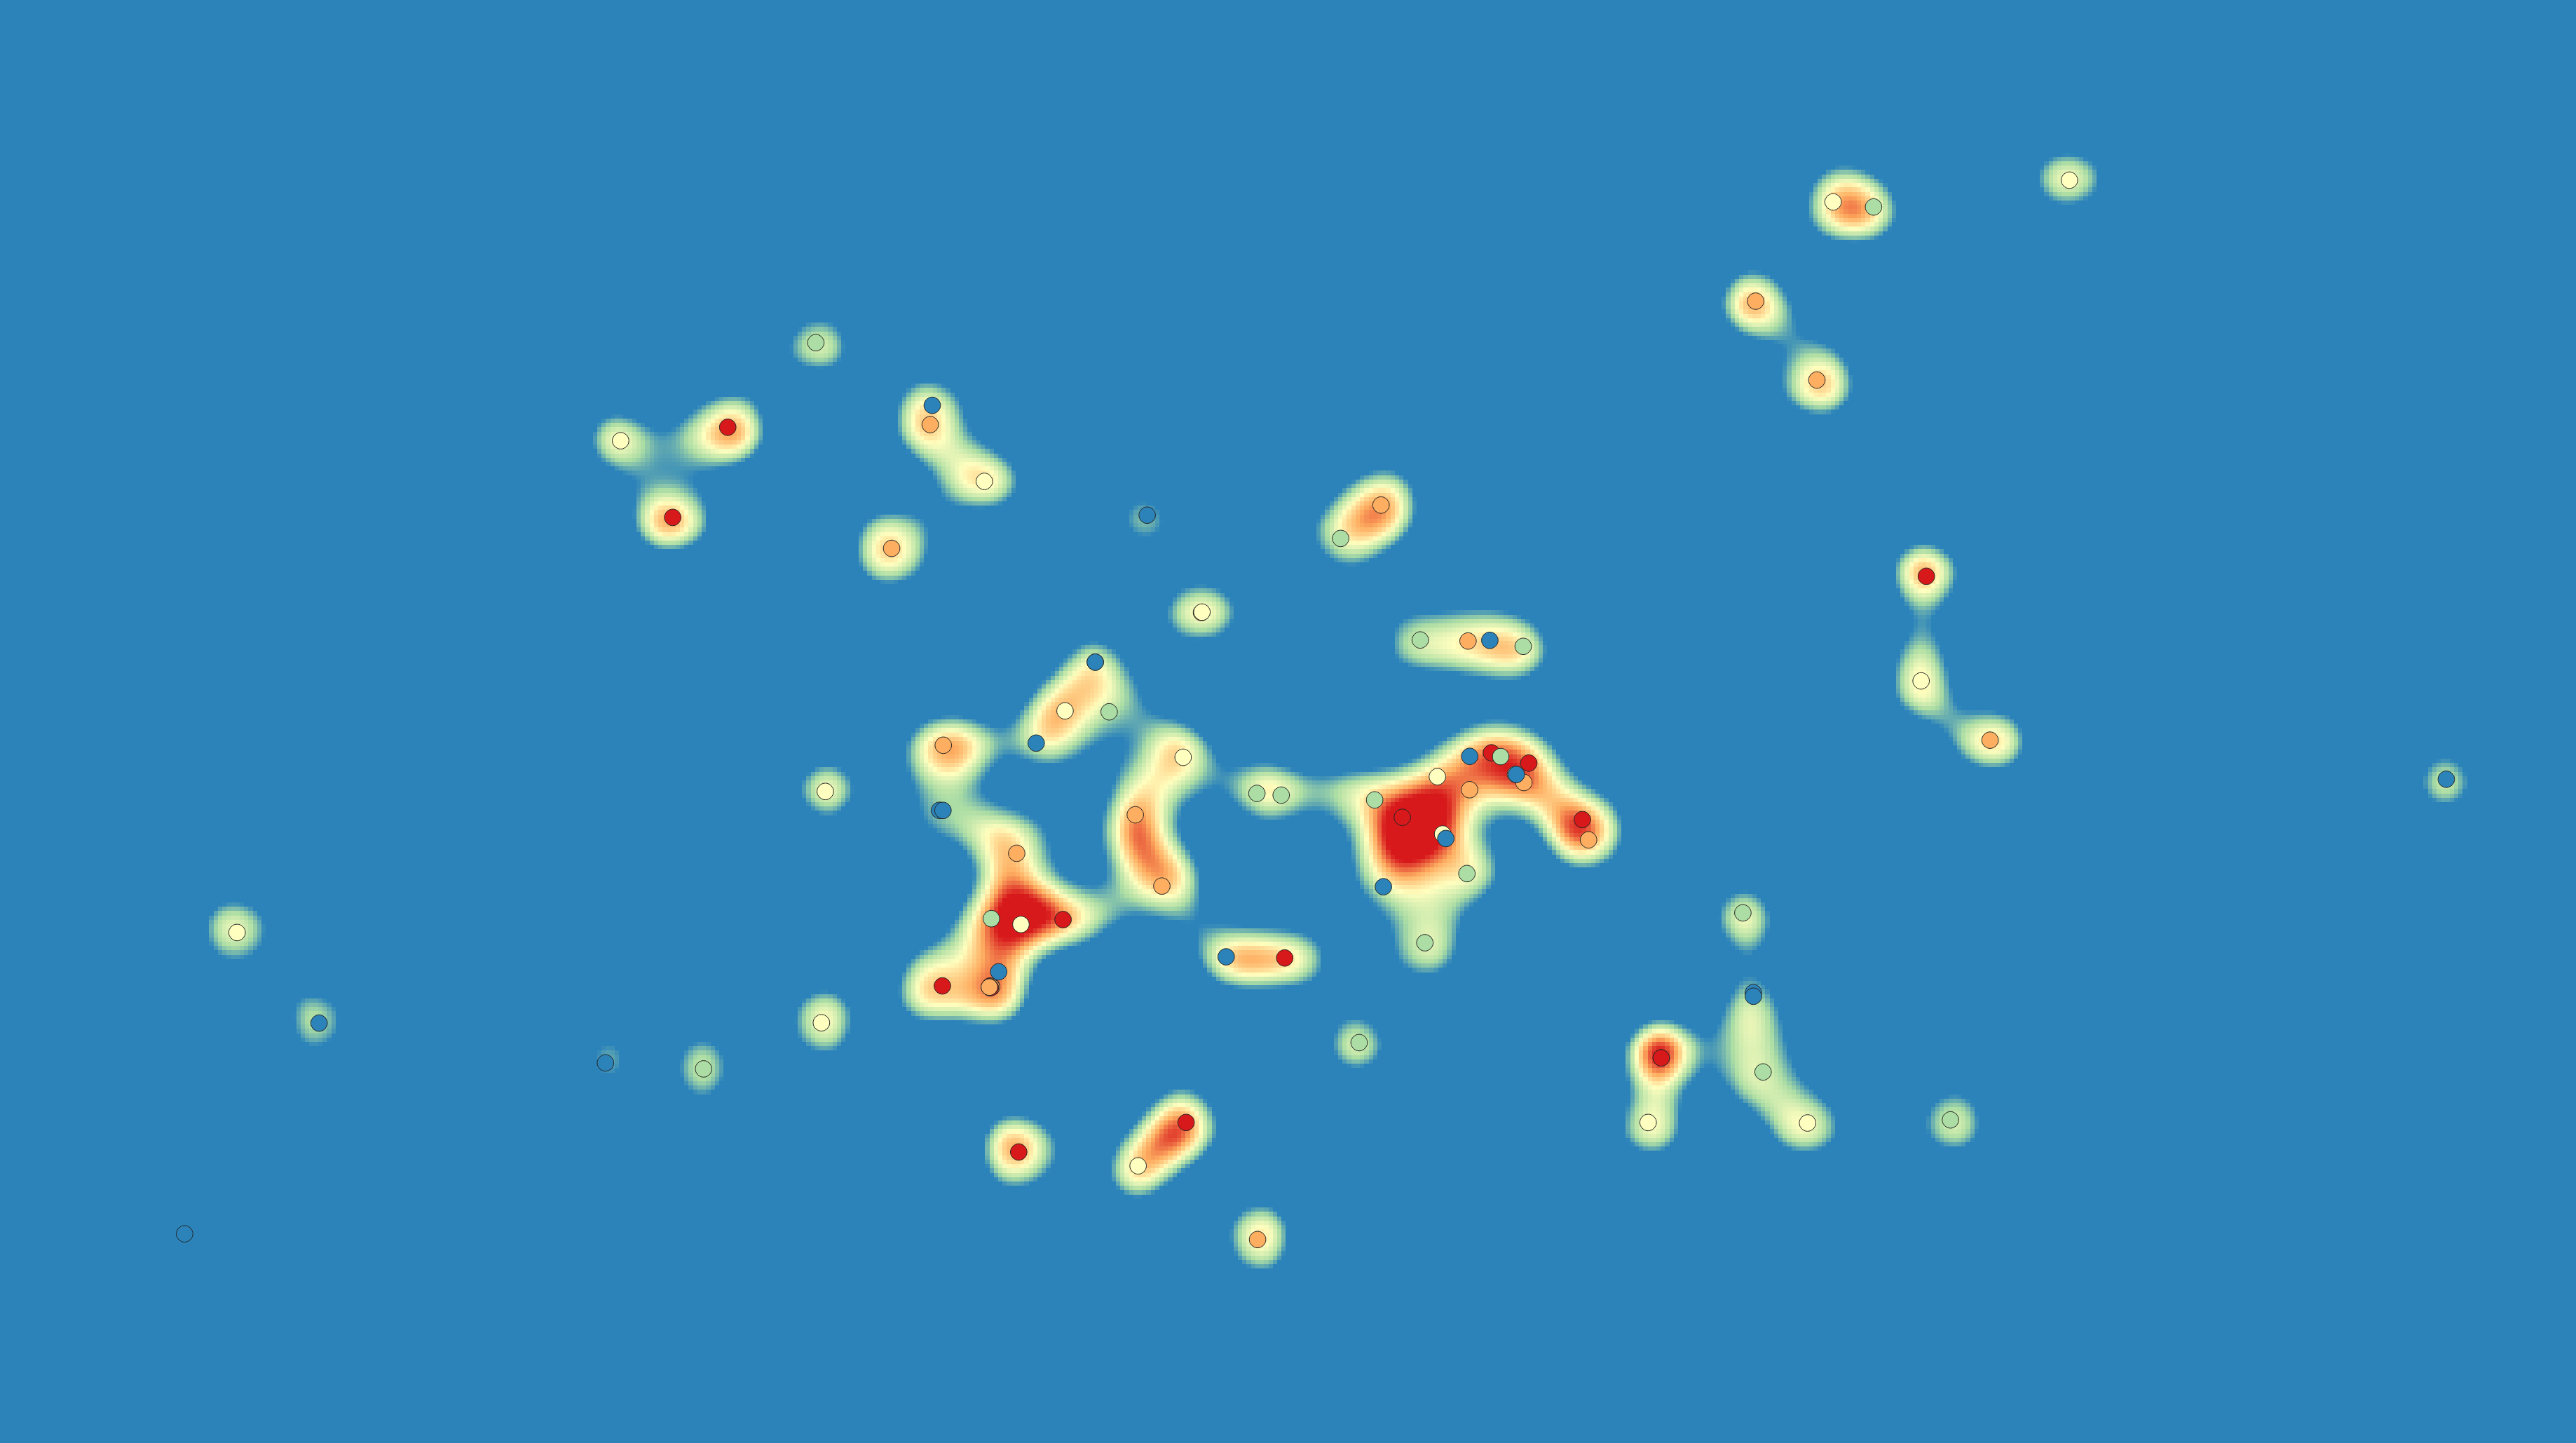
\includegraphics[width=.7\linewidth]{comparison/compare_bspline_saga.png}
	\caption{B-Spline interpolation using SAGA GIS}
	\label{fig:result_bspline}
\end{figure}

% !TeX root = ../document.tex

\section{Discussion}

In this study only local and small areas with occurring heat islands where detected. The \ldq{}heat islands effect\rdq{} was not set into context with the surrounding areas of Berlin, because we intended to focus on the intra-urban heat island effect only. Moreover, our decision was based on a lack of data outside the metropolitan area. Within the urban area the stations were evenly distributed as shown in figure \ref{fig:station_dsitribution} and are thus suitable for several of the interpolation methods. It should be emphasized that the stations are subject to different microclimates and as such are influenced by parks, large sealed areas or open water. \cite{chowienczyk_estimating_2020} Also, technical failure of the measuring instruments are possible and need to be taken into account. These effects were not studied in detail, but could have a significant impact on the results. Because detailed analysis of the stations, their location and immediate surroundings was not possible, the pre-processing of the raw data was an important step in order to receive more accurate and reliable data without outliers. Some of these outliers thus were identified and omitted in the further process. However, the reliability and accuracy of the data depends on and the choice of method for detecting and removing the outliers, which leaves some uncertainty and needs further evaluation. 

% TODO: Fix citation above
% TODO: Focus on answering: choice of data, aggregation and quality of data/ choice of method and parameters (power factor)/ discuss the results and differences 


\begin{figure}[H]
	\centering
	\includegraphics[width=.7\linewidth]{images/station_distribution.png}
	\caption{Distribution of sensor stations that measure the \ldq{}Temperatur\rdq{} phenomenon}
	\label{fig:station_dsitribution}
\end{figure}

\pagebreak
\appendix
\printbibliography

\end{document}
